\section{Chameleon IDE} \label{chameleon}

\chameleon{} comprises two parts: a type inference engine and an original debugging interface. This separate architecture allows us to 1) adapt \chameleon{} into multiple front ends, such as IDE extensions, desktop applications, and web applications, and 2) reuse the debugging interface for different programming languages by replacing the back end type inference engine. The debugging interface is designed from the ground up; the type inference engine is a re-implementation of the original Chameleon with several novel improvements.

\subsection{The Type Inference Engine}
\label{sec:typeinferenceengine}

Chameleon was originally a command-line tool developed in the early 2000s to improve type error reporting and introduced a design for interactive type debugging for the Haskell programming language. Unlike traditional type errors produced by the Glasgow Haskell Compiler (GHC)~\cite{ghc}, which uses a Hindley–Milner type inference system, Chameleon infers types using constraint solving. In Chameleon, Constraints are generated from the source code based on typing rules. In addition, each constraint is labeled with the location (line and column numbers) where it is generated. This set of constraints is consistent if the program is well-typed, inconsistent if otherwise. When a type error occurs, an efficient algorithm is used to derive a minimal subset of the constraints that still contains inconsistencies. This subset is called a Minimal Unsatisfiable Subset (MUS). From this, Chameleon can report a list of locations, using the labels of constraints that are in the MUS. Stuckey et al.~\cite{stuckey2003interactive} showed that program locations linked to the constraints from a MUS are all relevant to the type error and must include the cause of the error. In this paper, we will refer to these locations as \textit{error locations}.

Despite successfully borrowing the underlying ideas, we could not reuse the implementation of Chameleon due to the project language standard and libraries used was out of date. In addition to what Chameleon can do, a few new type inference features were added in the \chameleon{} implementation.



\paragraph{Recovering concrete types from type errors}


Using only constraints from the MUS is sufficient to locating the type error, but to recover types from type errors we need the constraints from parts of the program that irrelevant to the type errors.  For instance, consider an ill-typed 2-tuple where two possible types can be assigned: \texttt{(Int, Int)} and \texttt{(Int, String)}. The types reconstructed from Chameleon may be \texttt{(a, Int)} and \texttt{(a, String)}. Although the recovered types are theoretically correct, they introduce new type variable \texttt{a} making the error message harder to understand.  To solve this issue in \chameleon{}, we first expand the MUS to a maximally satisfiable subset. We do so by removing one constraint from the MUS to get a consistent set, and then repeatedly adding constraints from the global constraint store while maintaining consistency. This process stops when no more constraints can be added. The resulting subset, while not helpful to inform error locations, will produce the most concrete conflicting types. This difference can be seen in figure~\ref{fig:compare-to-original}. 


\begin{figure}[h]
    \centering
    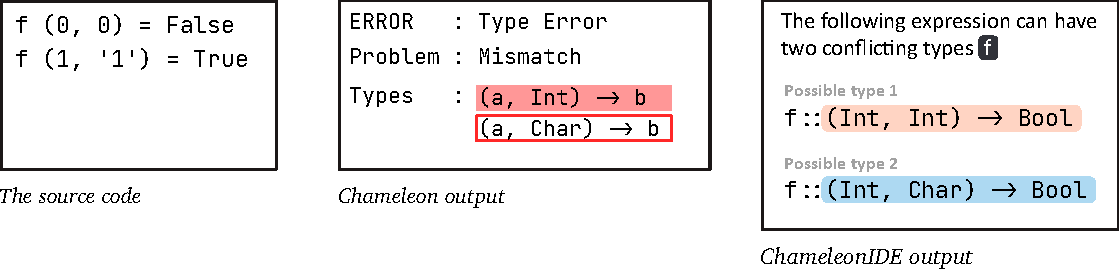
\includegraphics[width=\linewidth]{images/compare-to-original.pdf}
    \caption{
Reporting the same type error, Chameleon uses
\texttt{Int -> a} and \texttt{Char -> a}, while \chameleon{} uses the 
concrete types \texttt{Int -> Bool} and \texttt{Char -> Bool}.
    }
    \label{fig:compare-to-original}
\end{figure}

This has a few benefits. First, concrete types provide extra information to programmers. With a type of \texttt{(Float, Float)}, programmers may want to convey a point in 2d space. However, this information is not preserved in \texttt{(a, Float)}. Second, with concrete types, the debugging front end has more flexibility to change the representation of types. If the front end
understands the type language in Haskell, it is possible to recognize and replace ground facts that are overlapping in both possible types and have the same effect. The other direction is impossible. 

\paragraph{Type error explanation}

In addition, \chameleon{} provides support for type explanation. Similar to the type explanation system ~\cite{jun2002explaining} from Yang,  \chameleon{} is able to produce a human-readable explanation, but for type errors. This is achieved by expanding the metadata fields of each constraint to contain the information needed for type explanation. 

\begin{lstlisting} [
    language=Haskell, caption={
    A simple program that is ill-typed. This program generates two constraints from line 1 and one constraint from line 2.
}, label={listing:ifelse}
]
if a then b else c
a = "True"
\end{lstlisting}
For instance, the program in the listing \ref{listing:ifelse} \chameleon{}  generates the following constraints and labels (in brackets) $T_a = Bool$ (if condition), $T_b = T_c$ (if branches), $T_a= String$  (definition). Clearly, as $T_a$ can not unify with both \textit{Bool} and \textit{String}, this program is not well typed. \chameleon{} can construct a human-readable explanation from the MUS, for example: \texttt{a} has type \texttt{Bool}, because \texttt{a} is the condition of an if statement; however \texttt{a} has type \texttt{String}, because \texttt{a} is defined as the string literal \texttt{"True"}. This low-level explanation is used in a high-level user interface described in section \ref{sub:deduction-steps} to help programmers reason about the validity of error locations.


\begin{figure}[h]
    \centering
    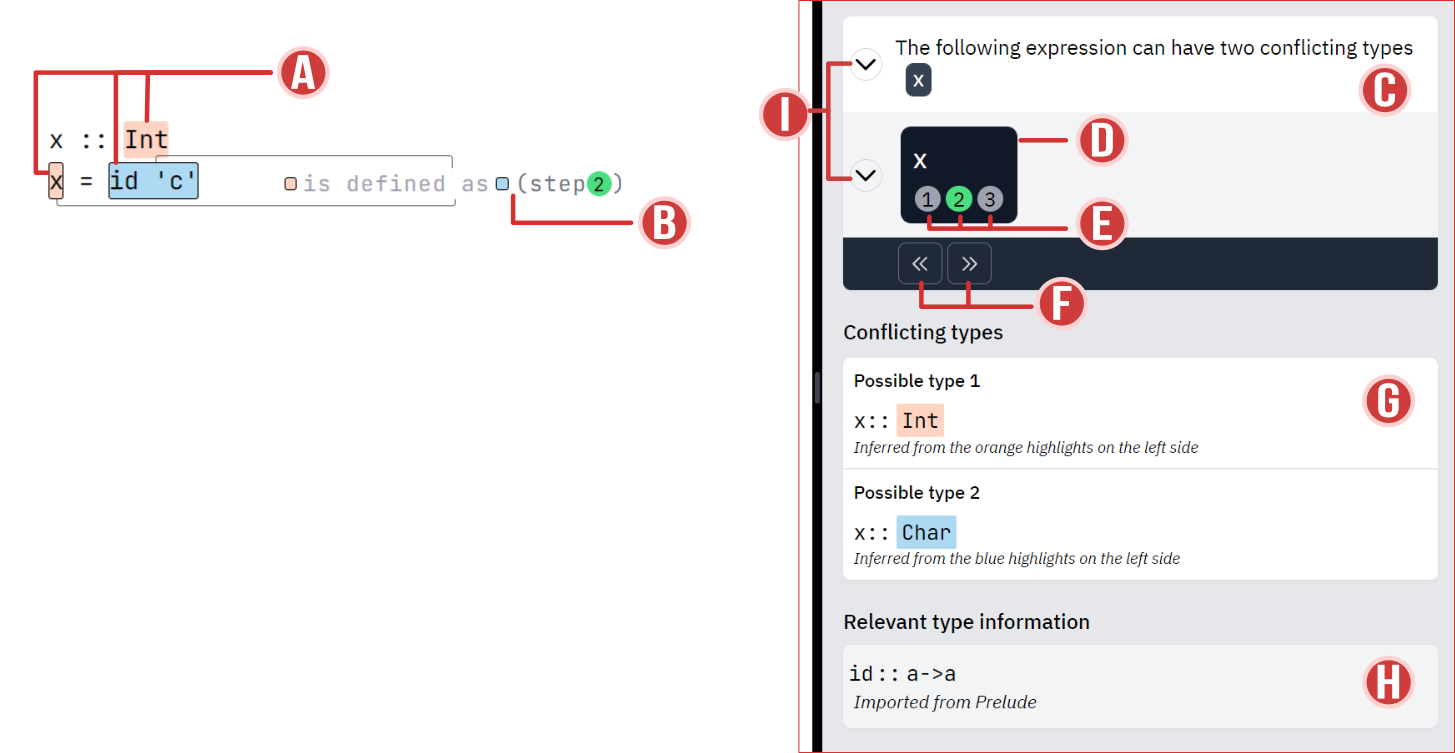
\includegraphics[width=\linewidth]{images/atonomy.png}
    \caption{
        \textbf{The anatomy of \chameleon{}.}
        \chameleon{} consists of two windows: an editor window on the left and a
        debugging window on the right. The editor window is similar to a
        traditional code editor. Fragments of source code may have a highlight
        color (A). Additionally, an explanation layer (B) displays in the editor
        window, if deduction steps are enabled. The debugging window contains
        three panels. A message panel contains an error description (C), and, optionally,
        a list of candidate expression cards (D), a list of deduction steps (E), 
        and a control bar (F) to increment/decrement deduction step. 
        The conflicting types
        panel (G) shows two possible types inferred by the type inference
        engine. A relevant type information panel to show additional information
        that may help understand type errors.
    }
    \label{fig:anatomy}
\end{figure}


\subsection{The Debugging Interface}

The \chameleon{} debugging interface provides three main features to visualize the relation between an error statement and the error locations in the source code, and to explore the explanation of each error location given by the type inference engine. Further, programmers  can turn on and off features to suit their preferences and debugging needs.



\paragraph{Type compare tool} \label{sub:type-compare}

The type compare tool shows the two conflicting types in different colors, each associated with one or more error locations (Fig. \ref{fig:compare}).  The type error must be fixed by modifying at least one of these locations. The error locations are highlighted with the matching color of the conflicting types. The type compare tool is useful to quickly bisect the type error. If the programmers know the expression's intended type (they usually do), they will be able to eliminate half of the possible locations. To make the bisecting effect more pronounced, a user can hover on one of the possible types and only show the relevant locations that
contribute to that type. This is a convenient way to put the error "under the spotlight".


\begin{figure}[h]
    \centering
    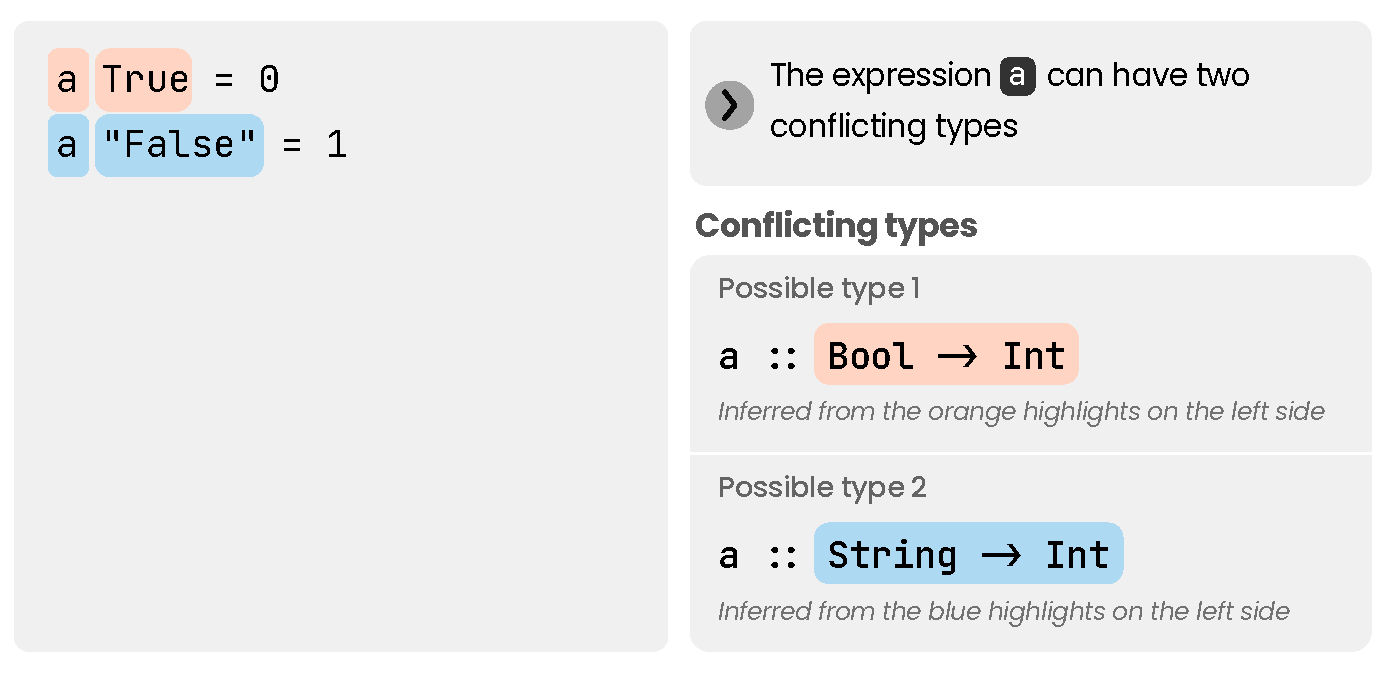
\includegraphics[width=\linewidth]{images/intro-compare.pdf}
    \caption{
        \textbf{\chameleon{} minimal output (with candidate expression cards and deduction step disabled)}. \chameleon{} identified the conflicting types for the function \texttt{a} and associated the relevant locations with each type. In addition, \chameleon{} leaves out the right-hand side of the declaration '\texttt{0}' and '\texttt{1}' because they are unrelated.
}
    \label{fig:compare}
\end{figure}

\begin{figure}
    \centering
    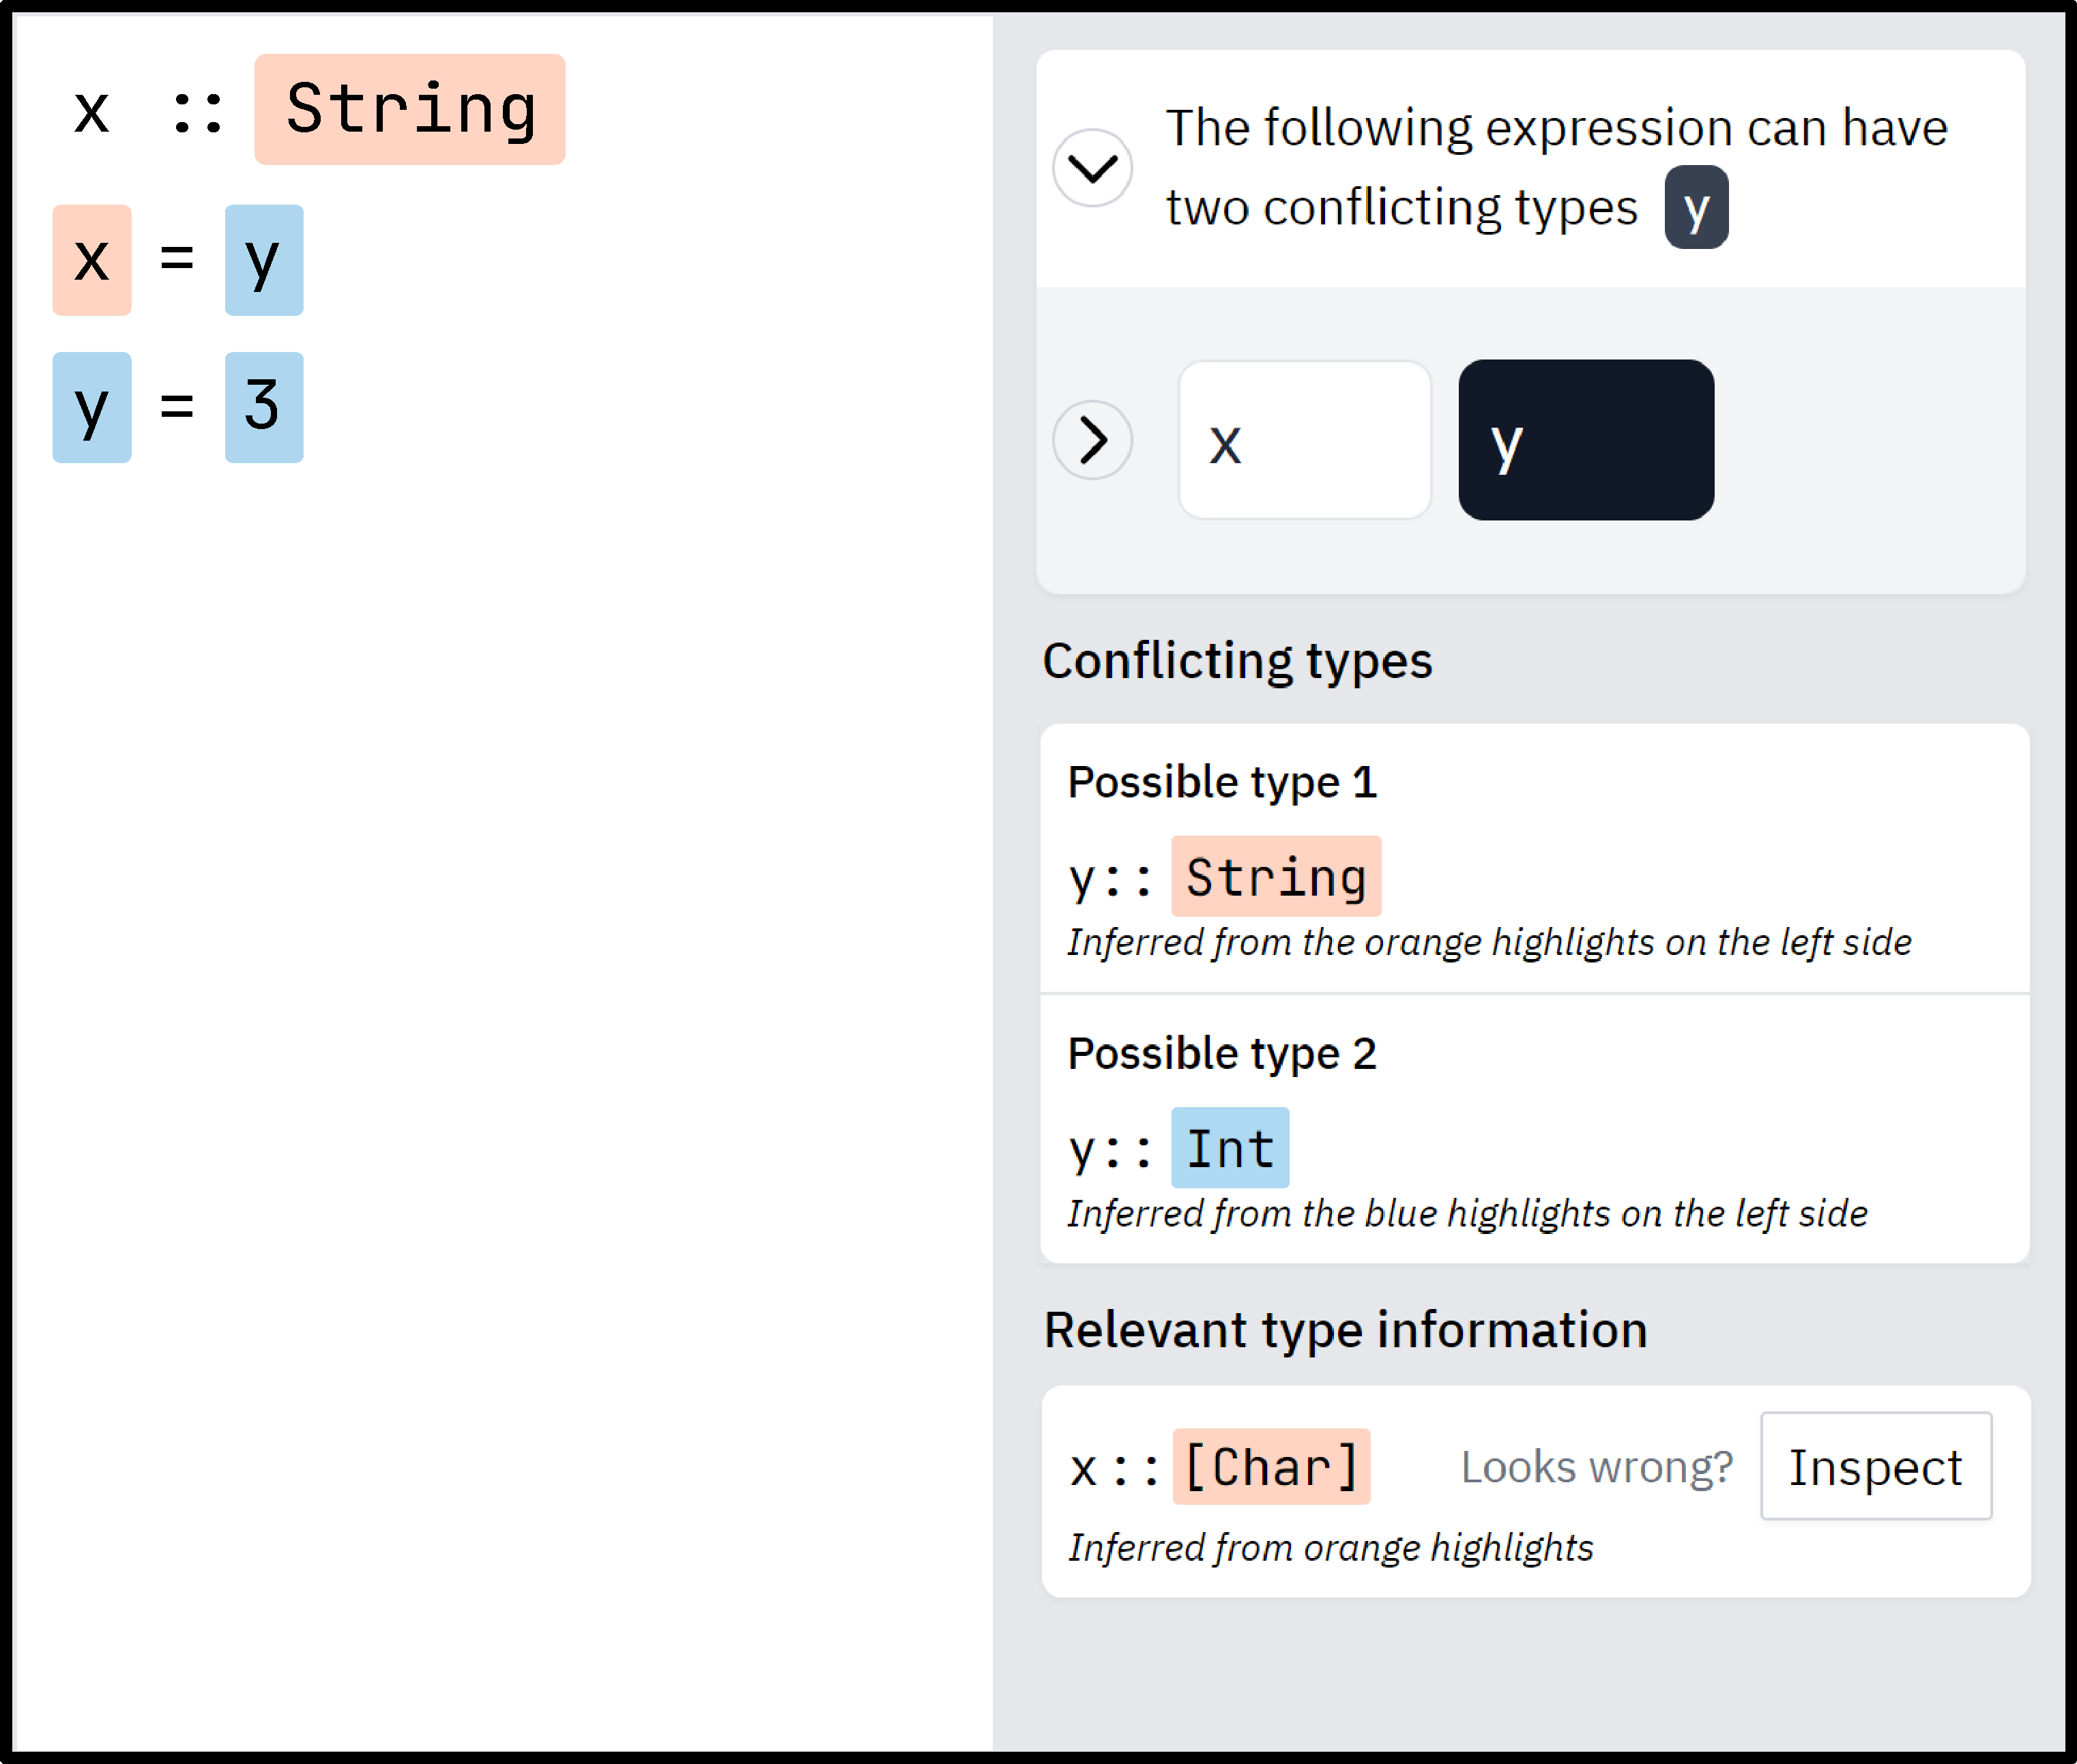
\includegraphics[width=\linewidth]{images/intro-expression.pdf}
    \caption{
        \textbf{\chameleon{} with only candidate expression cards enabled.}
        \chameleon{} shows that the type error can
        occur in the definition of '\texttt{x}' or '\texttt{y}'.
    }
    \label{fig:expression}
\end{figure}


\begin{figure}
    \centering
    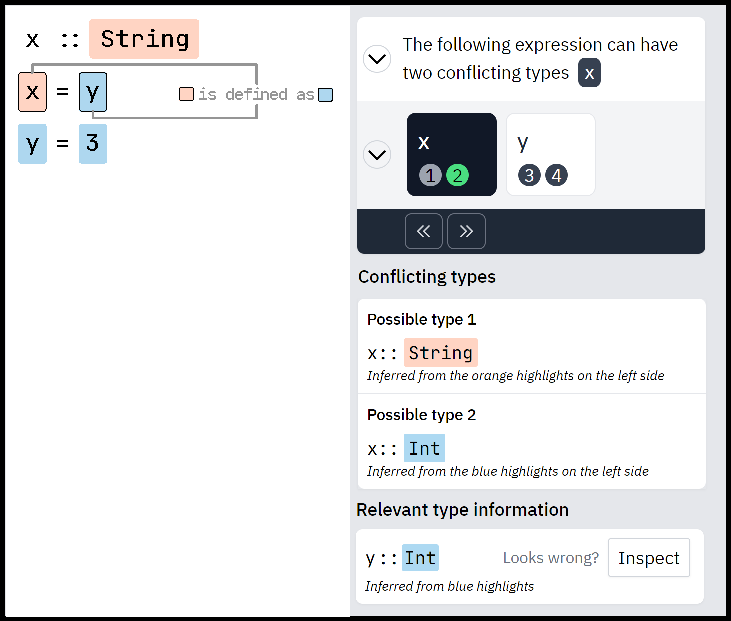
\includegraphics[width=\linewidth]{images/intro-deductionstep.pdf}
    \caption{
        \textbf{\chameleon{} with both candidate expression cards and deduction steps
        enabled.}
        \chameleon{} explains the type error in four steps. In the screenshot, the active step is step 2, where \chameleon{} shows that the expression \texttt{x} and \texttt{y} should have the same type. 
    }
    \label{fig:deduction}
\end{figure}



\paragraph{Candidate Expression Cards}  \label{sub:candidate-expression}

A candidate expression is an expression that can be inferred to have two conflicting types. 
We propose candidate expression cards to make it clear to the user that there are multiple ways to resolve a type conflict. By contrast,  standard compiler error messages such as those of GHC arbitrarily focus the users attention on only one candidate expression, e.g.\ ``\textit{Couldn't match expected type ‘Char’ with actual type ‘Bool’ in expression x}" here x is the candidate expression. In practice this candidate expression often does not match programmers' intention (Fig. \ref{fig:single-candidate}).  

When a type error is detected, \chameleon{} provides a list of all candidate expressions and programmers are free to choose the problem to resolve by clicking on one candidate expression card. In the example shown in Fig. \ref{fig:expression}, \texttt{x} and \texttt{y} are both candidate expressions. Indeed, fixing one type error will make both expressions well-typed.


\begin{figure}[h]
    \centering
    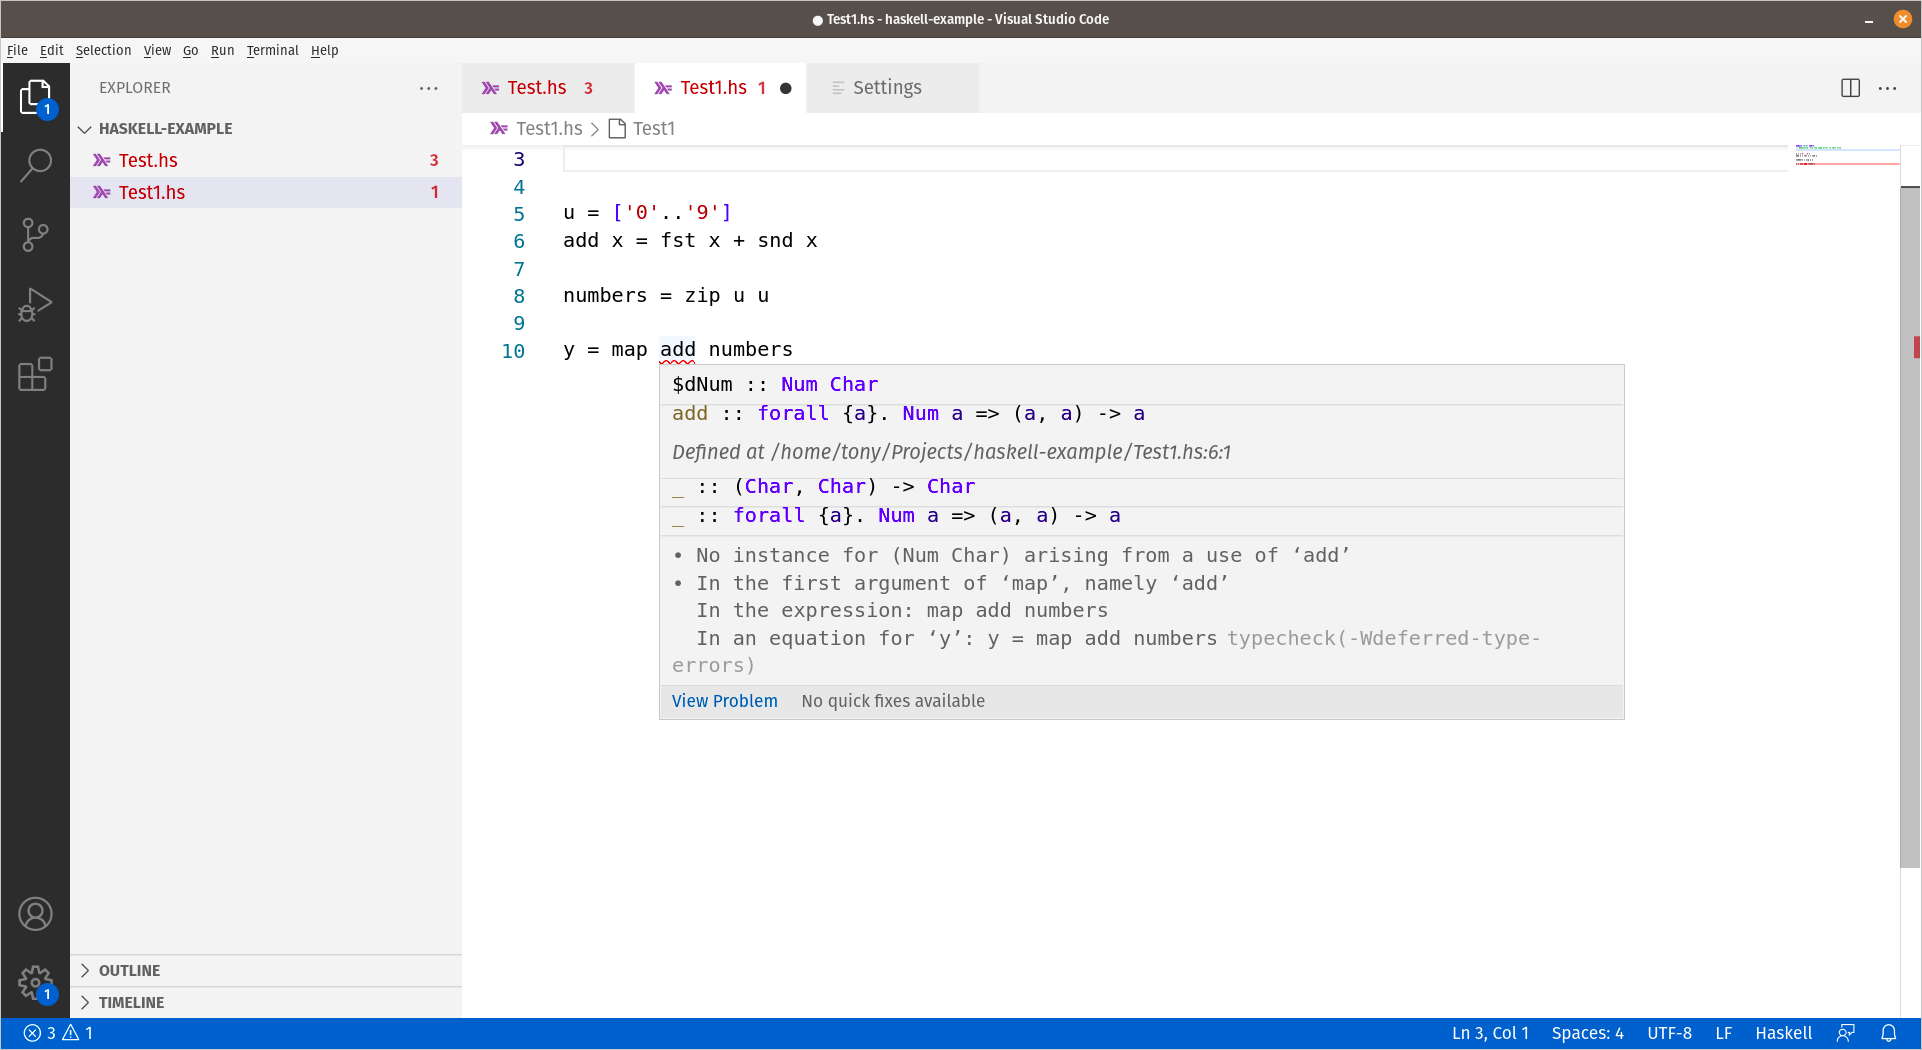
\includegraphics[width=\linewidth]{images/single-error-location-example.png}
    \caption{
With traditional type error messages, one expression is blamed for causing the type error. This expression may not always match the programmers' intention. 
    }
    \label{fig:single-candidate}
\end{figure}

Selecting a candidate expression card is a way for programmers to communicate to the type checker the knowledge that the other candidate expressions are in fact well-typed. Once a card is selected, the information in the conflicting types panel changes according to the change of candidate expression. In the editor window, some error locations change highlight colors to reflect the updated knowledge of the program. 


This feature can be effective in resolving the problem that traditional tools tend to report errors that happened in source code from third party libraries. With candidate expression cards, a programmer can freely change the context of the type error to the user defined variables and functions to gain a better understanding of why her own code does not match the library code instead of the other direction.


Programmers interact with the candidate expression cards by clicking on them to commit the change of meaning or hovering on them to peek at the effect of the change; the effect is reverted once the cursor moves away.


\paragraph{Deduction steps}  \label{sub:deduction-steps}

Deduction steps are motivated by the lack of explain why the program has  type errors. When compiler reject a program, it dumps the internal state of type checking.  This information may be a result of complex computing but this process is not reported by compilers. For a typical type error shown in Fig. \ref{fig:ghc-error-example}, clearly the evidence for type error are gathered from are generated from the previous two declarations. These have to be re-discovered by the programmers again, using harder and less sound methods. 

\begin{figure}[h]
    \centering
    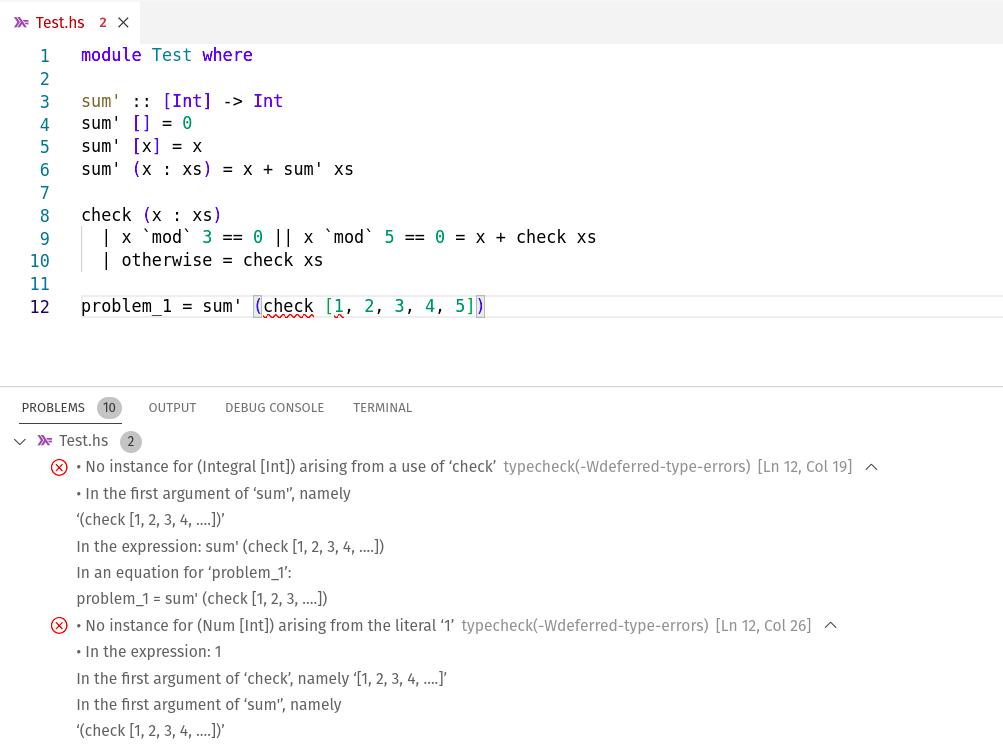
\includegraphics[width=\linewidth]{images/ghc-error-example.png}
    \caption{
        }
    \label{fig:ghc-error-example}
\end{figure}

Deduction steps allow programmers to explore all the error locations one at a time (Fig. \ref{fig:deduction}). Steps are shown as a list of sequentially  numbered circular buttons (step buttons) and an explanation layer in the editor window. In the explanation layer, two highlighted error locations are outlined, and a line is drawn to connect these two locations to a human-readable text explanation of
their semantic connection. Programmers are free to activate any step. The active step is shown as the green button. When activating a step, some highlights switch color. The message in the explanation layer changes as well. A program in Fig. \ref{fig:deduction} generates a list of steps shown in Fig. \ref{fig:step-interface} left.

Programmers use their mouse and keyboard shortcuts to increment or decrement the step number or jump to any step. Typically, a programmer resolves  type errors by navigating through all the deduction steps and verifying whether each explanation aligns with the intended meaning of the program. Eventually, she will find a step that does not match her intention, and the type error can be fixed by modifying one of the two outlined error locations.


\begin{figure}[h]
    \centering
    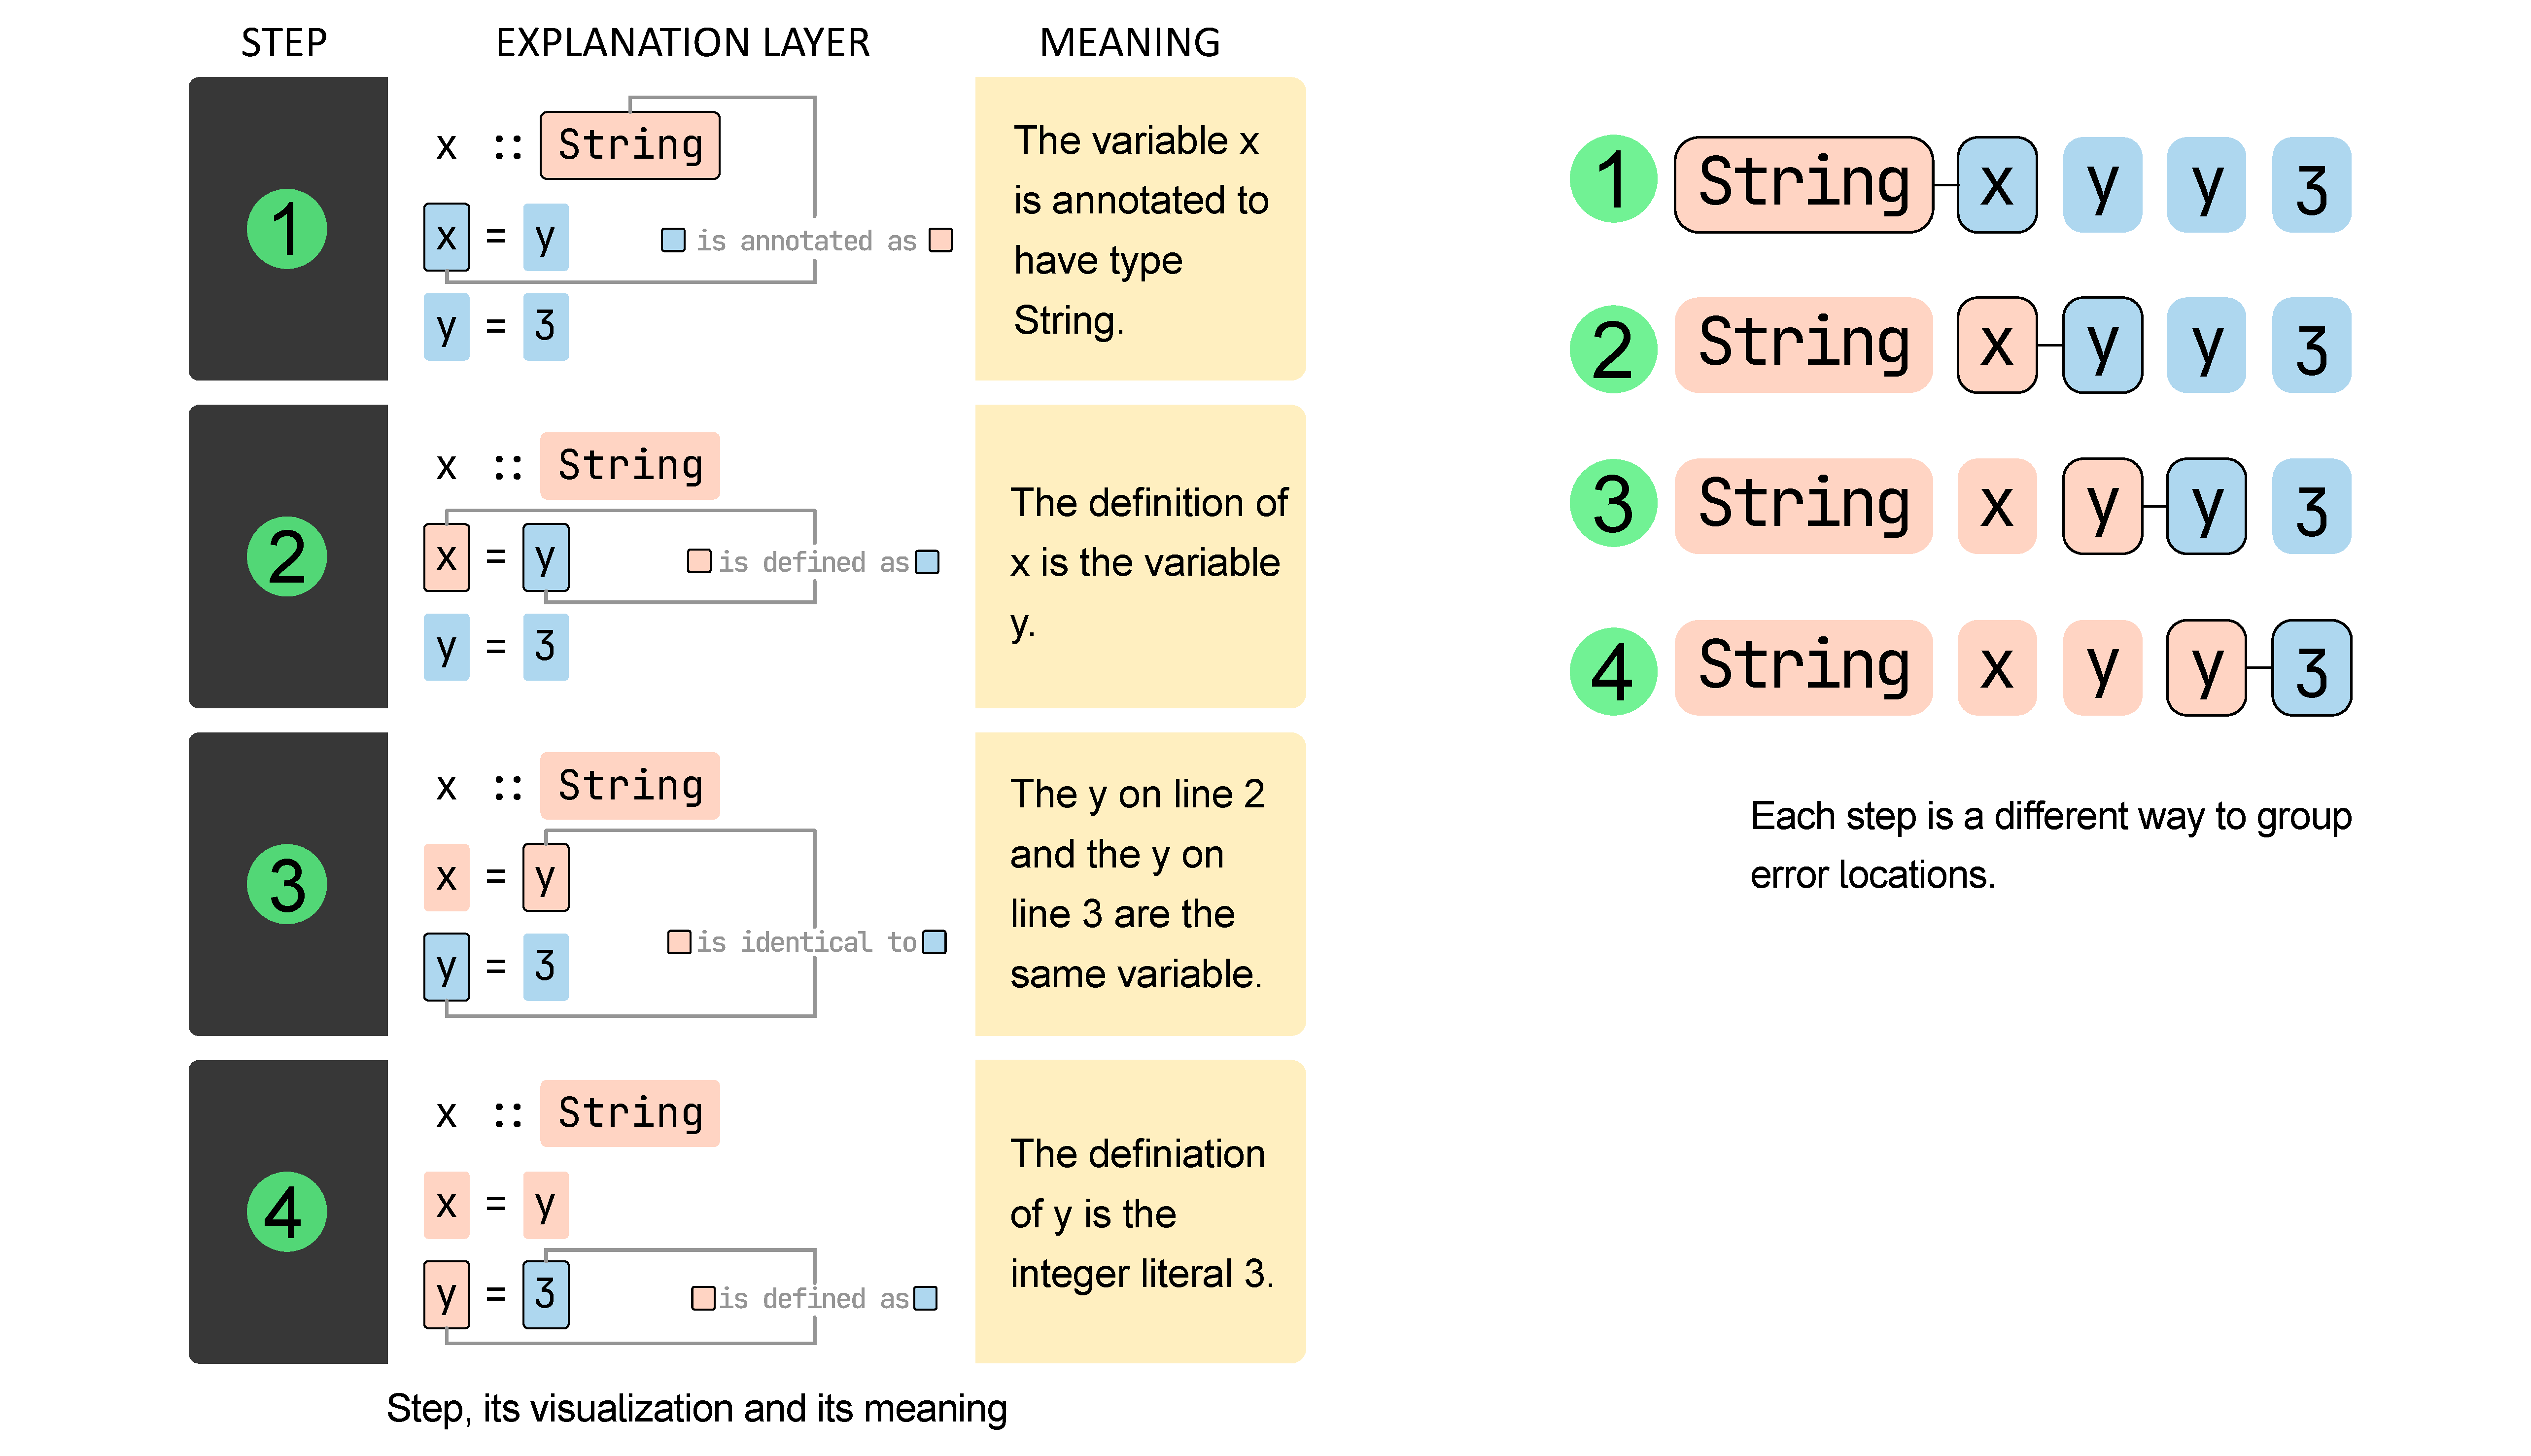
\includegraphics[width=\linewidth]{images/step-interface.pdf}
    \caption{
Deduction steps if they are shown all at once (left). In practice, steps are shown one at a time. Programmers increment or decrement the step number using the step control bar (Fig. \ref{fig:anatomy}-F) or by directly clicking on a step button (Fig. \ref{fig:anatomy}-E). To increment or decrement the deduction step can be intuitively thought of as to move the position of the \textit{split point} where the blue and orange highlights divide (right).
        }
    \label{fig:step-interface}
\end{figure}

Internally, deduction steps are different ways to group the error locations into two different highlighted colors. If all the highlights are placed in a list-like data structure, each increment of the step numbers moves the end of one color and the start of the other forward (Fig. \ref{fig:step-interface} right).


\paragraph{Multiple Modes}

Nielson pointed out \cite{nielsen1994usability}  that the two most important issues in designing for usability are understanding the users' tasks and the differences in users. From analyzing how users use \chameleon{}, we realized that the ideal debugging interface should adapt to the specific programmer and programming task. It is common that a programmer wants the debugger to just "show the answer", and it is also possible a programmer wants to dive deeper into the problem domain and search for the optimal solution. To accommodate the need to customize the level of information density and granularity of control, \chameleon{} provides three modes: basic, balanced, and advanced. Programmers can switch between modes by clicking on the mode switching toggles (Fig. \ref{fig:anatomy}-I). The features accessible from different modes are shown in table~\ref{tab:chameleon-features}.

\begin{table}
    \centering
    \begin{tabular}{ l l  }
     Mode & Features \\ \hline
     Basic Mode & Type Compare Tool \\ \hline
     Balanced mode & Type Compare Tool \\
     & Candidate Expression Card \\  \hline
     Advanced mode & Type Compare Tool \\
     & Candidate Expression Card \\
     & Deduction Steps \\
    \end{tabular}
    \caption{\chameleon{} modes and features}
    \label {tab:chameleon-features}
\end{table}


